\indent Acorde a lo solicitado, mostraremos distintos tipos de familias de casos para nuestro algoritmo, y adem\'as, daremos el tiempo estimado 
seg\'un la complejidad del algoritmo calculada anteriormente.\\

A continuaci\'on mostraremos un gr\'afico de tiempos comparativo entre distintas familias de casos:\\ 

\vspace*{0.3cm} \vspace*{0.3cm}
  \begin{center}
 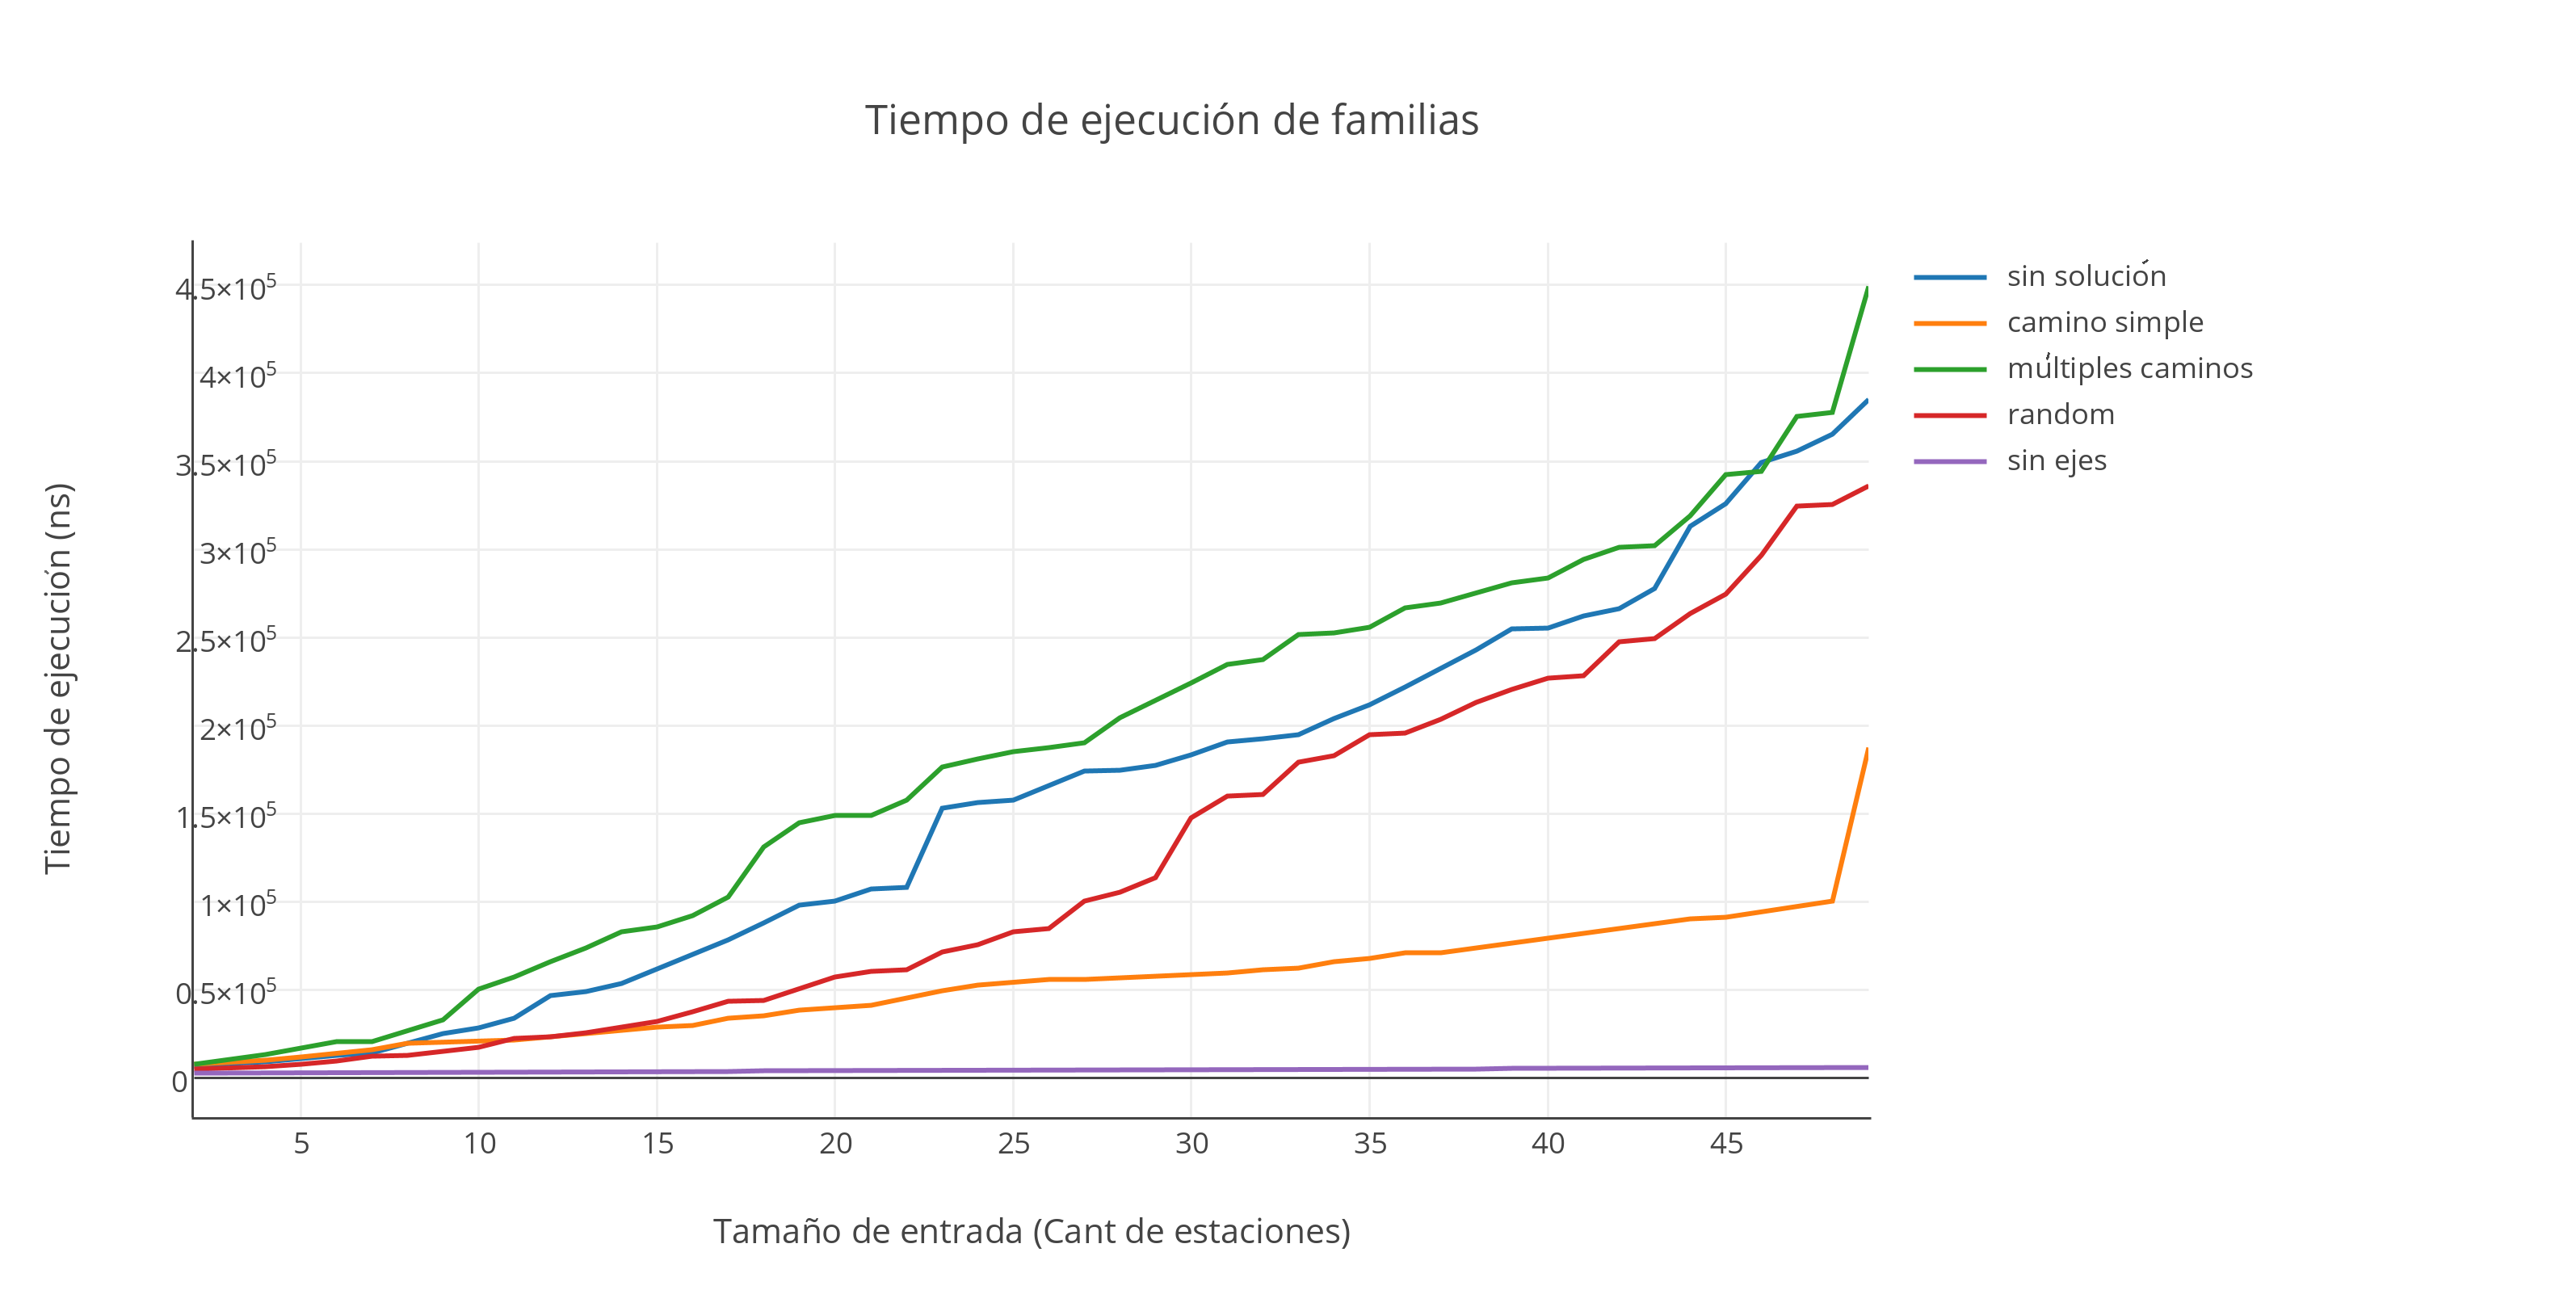
\includegraphics[scale=0.65]{./EJ3/comparativo.png}
 {$Gr$\'a$fico$ \ 3.1 - $Comparativo$}
  \end{center}
  \vspace*{0.3cm}
  
Se puede observar en el gr\'afico, cuatro funciones las cuales representan el tiempo de ejecuci\'on de las familias de casos:\\
\begin{itemize}
\item Sin solución
\item Sin ejes
\item Camino simple
\item Múltiples caminos de igual peso llegan a destino
\item Random
\end{itemize}

Como se observa en el gr\'afico la funci\'on representativa de la familia n\'umero 2, presenta una mejor performance en relaci\'on a las otras. Esto se debe a que nuestro algoritmo intenta chequear las aristas para armar los caminos y como encuentra que no hay ningun camino de ningun nodo hacia otro finaliza su ejecuci\'on demandando unicamente la creaci\'on del grafo.

Luego de chequear dichas instancias, pudimos llegar a la conclusi\'on que la familia de casos que presenta una mejor performance para nuestro algoritmo
es en el cual \textbf{No hay ejes, todos los nodos desconectados}

Un grafo representativo de lo dicho ser\'ia el siguiente:

\vspace*{0.3cm} \vspace*{0.3cm}
  \begin{center}
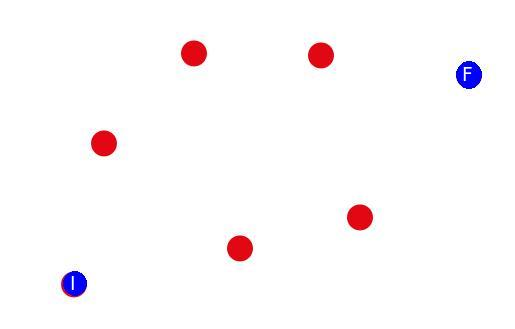
\includegraphics[scale=0.5]{./EJ3/grafoSinEjes.jpeg}
\\{$Grafo$ \ 3.1 - $Mejor$ $Caso$} 
  \end{center}
  \vspace*{0.3cm}
  
Para llegar a dicha conclusi\'on trabajamos con 50 instancias.\\

Para una mayor observaci\'on desarrollamos el siguiente gr\'afico con las instancias:\\

\vspace*{0.3cm} \vspace*{0.3cm}
  \begin{center}
 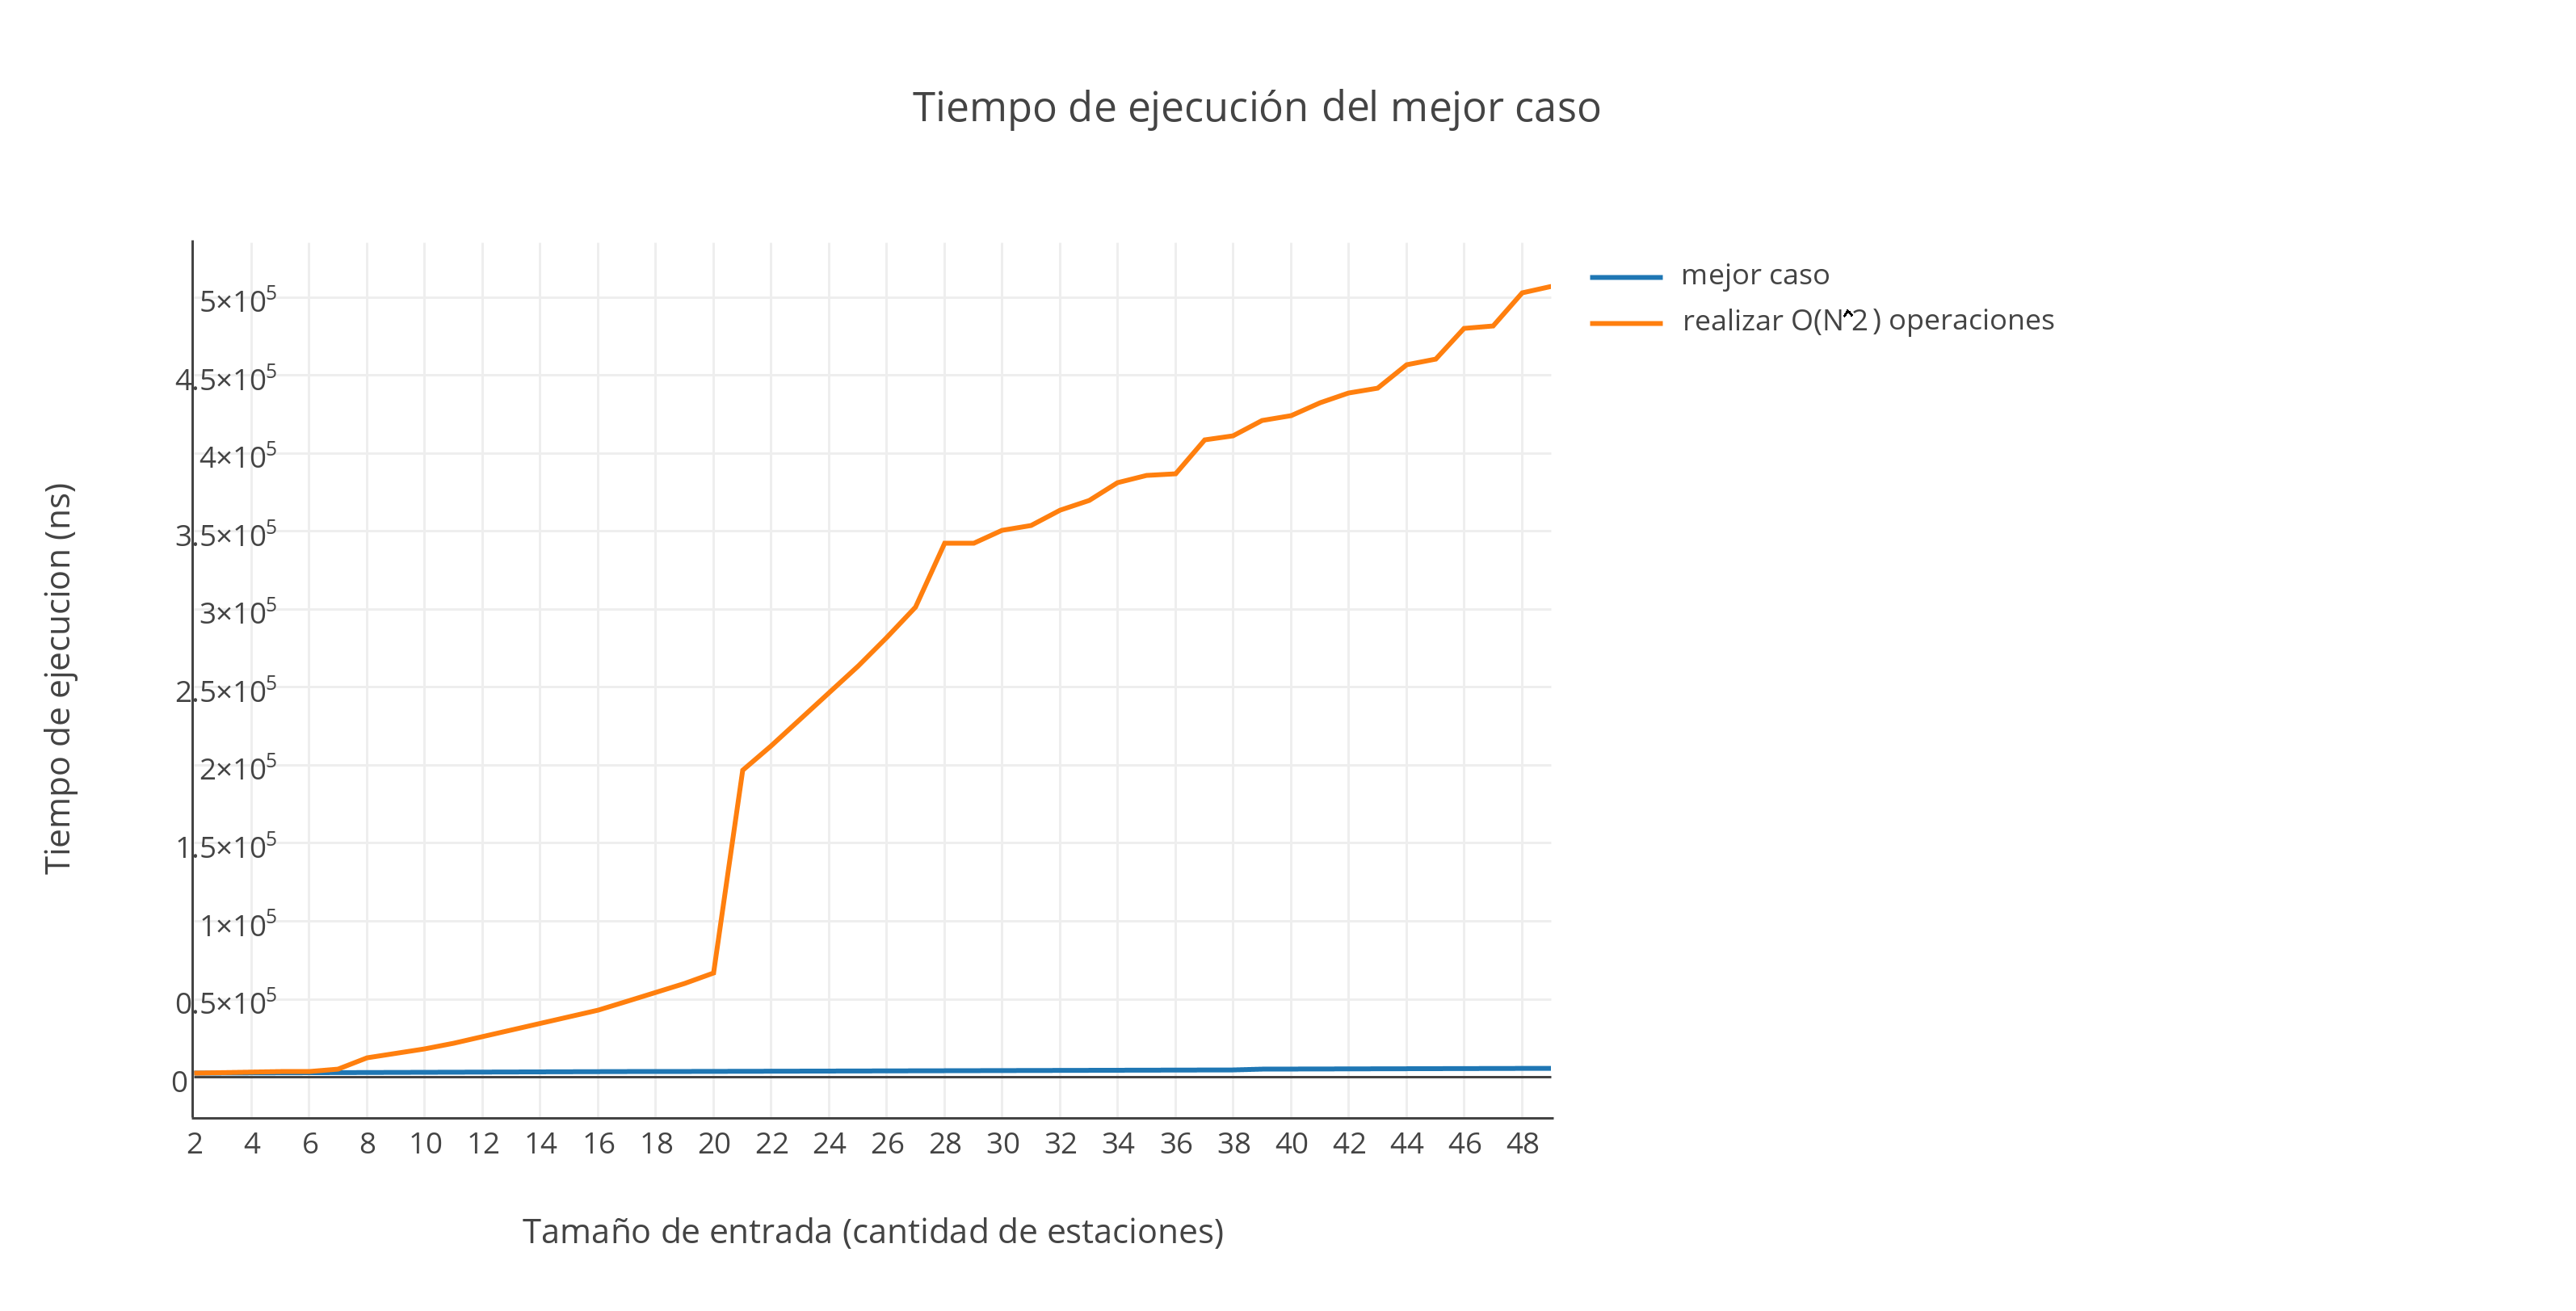
\includegraphics[scale=0.65]{./EJ3/mejorcaso.png}
 {$Gr$\'a$fico$ \ 3.2 - $Mejor$ $Caso$}
  \end{center}
  \vspace*{0.3cm}
  
Como es posible observar en el gr\'afico, la funci\'on resultante de la cota teorica crece mucho m\'as r\'apido que la de nuestro algoritmo la cual queda considerablemente por debajo . Es por esto que graficamos el mismo contra la funci\'on de $O(N*k) con k < N$

\vspace*{0.3cm} \vspace*{0.3cm}
  \begin{center}
 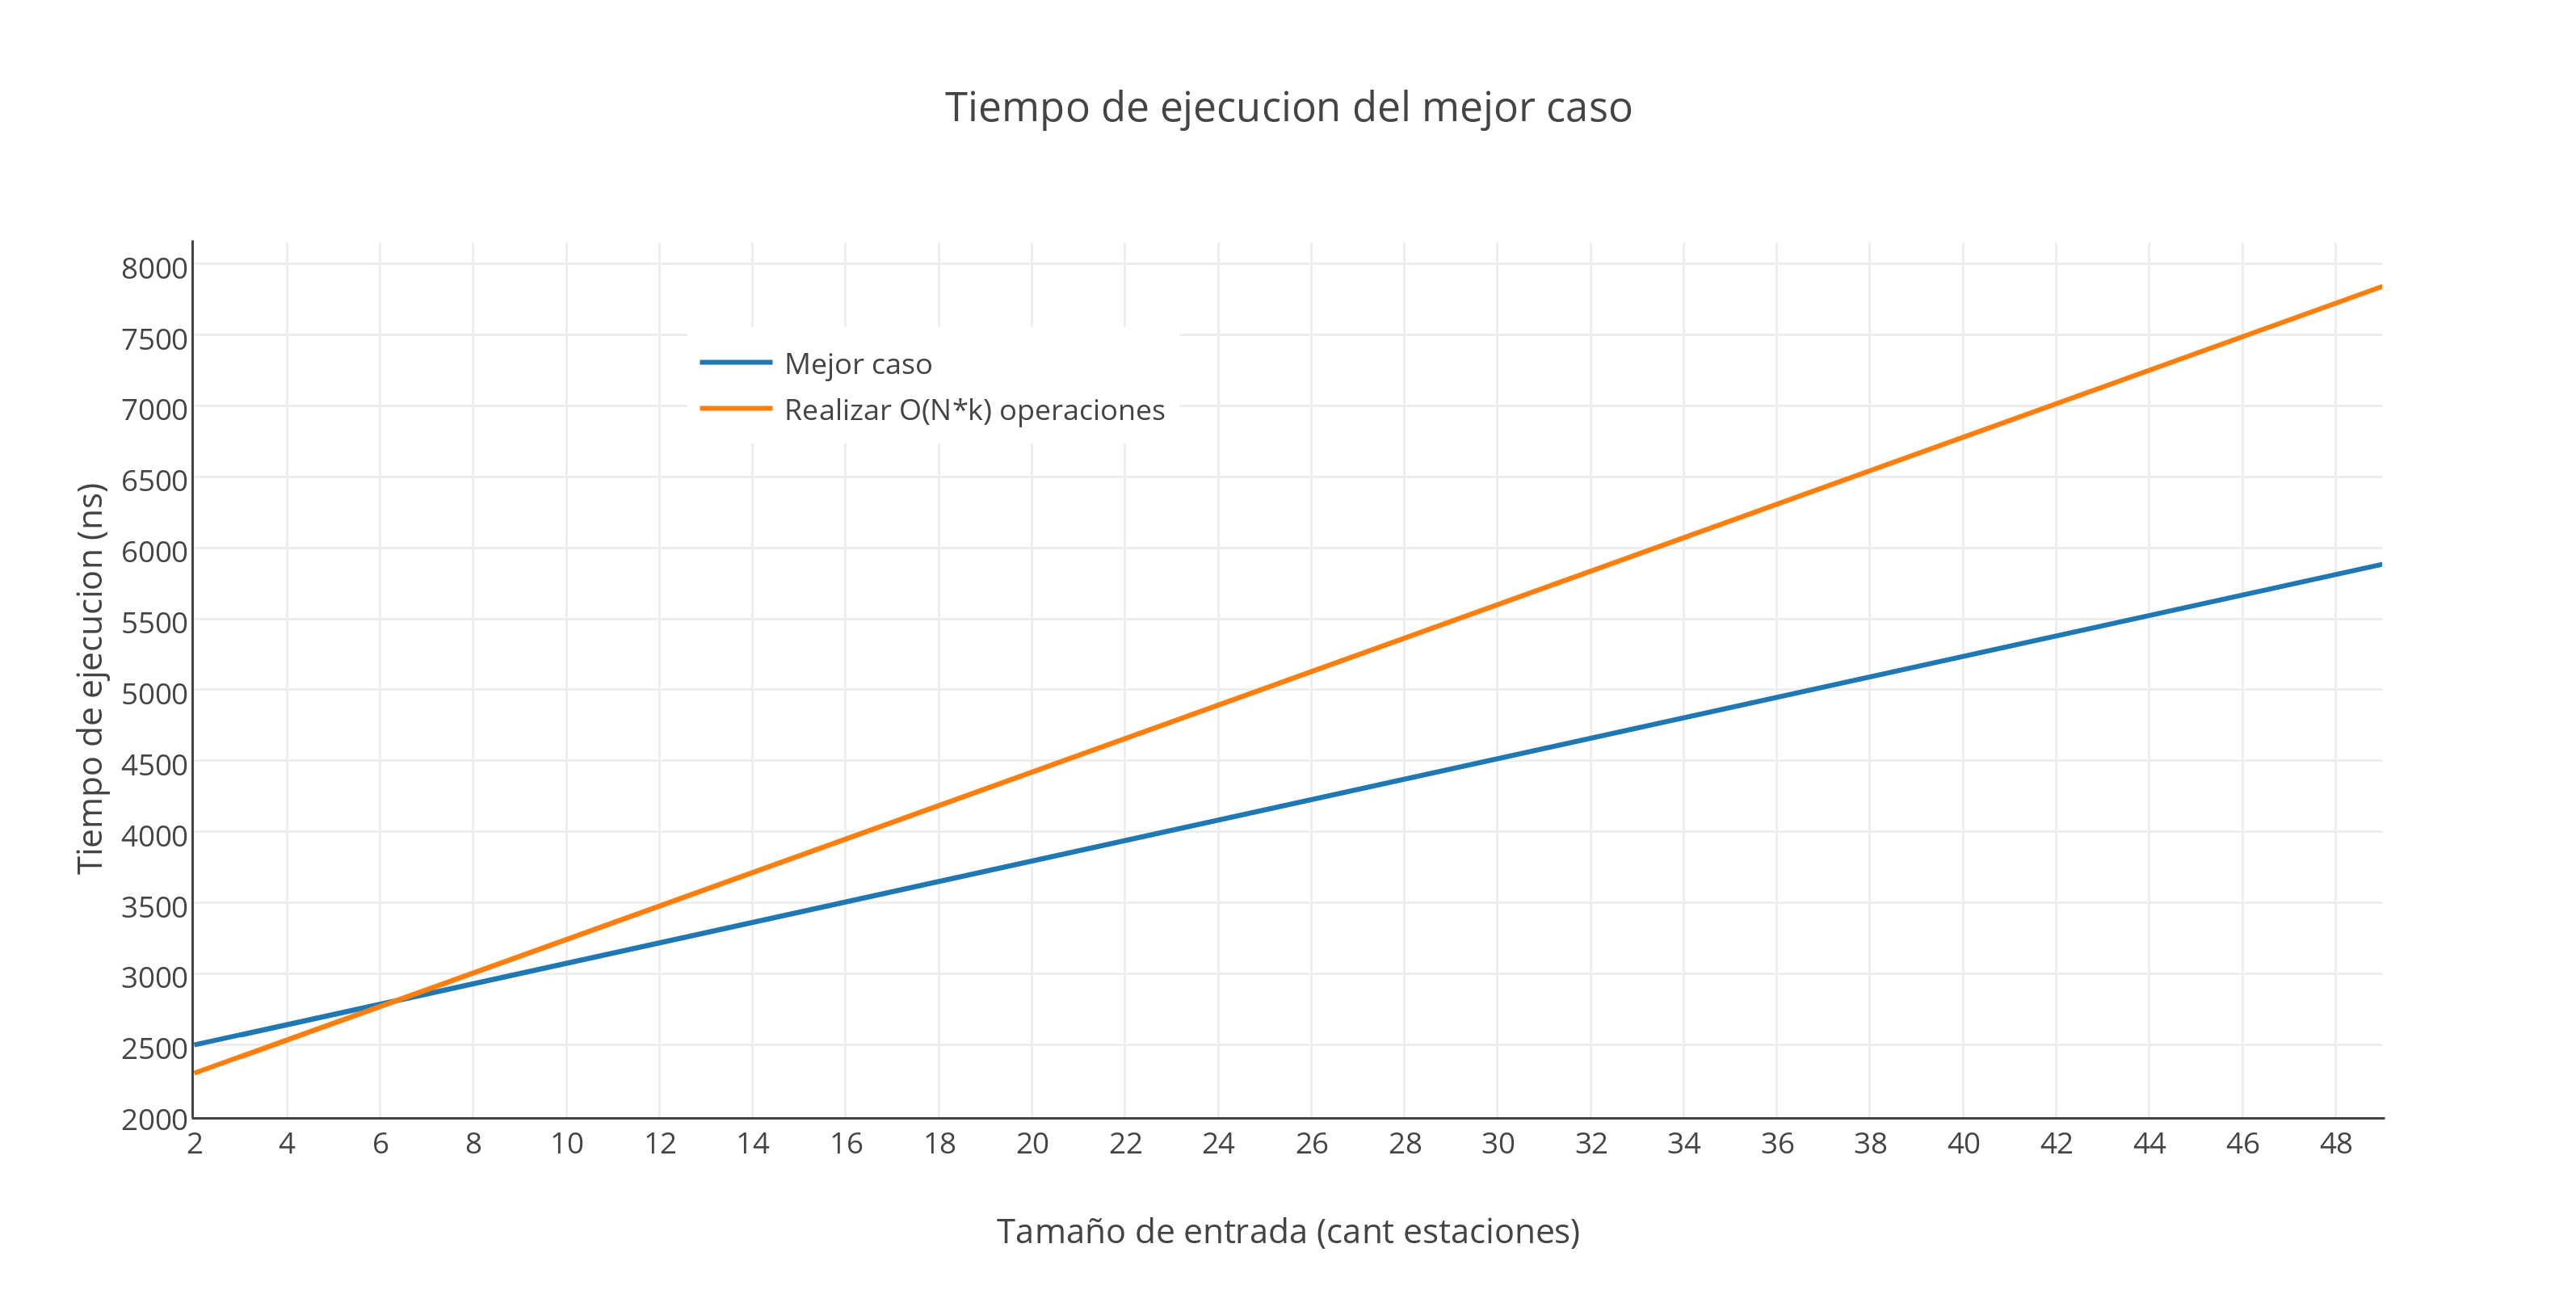
\includegraphics[scale=0.65]{./EJ3/mejorcaso1.png}
 {$Gr$\'a$fico$ \ 3.3 - $Mejor$ $Caso$}
  \end{center}
  \vspace*{0.3cm}


Se puede observar como la funci\'on resultante de realizar O(N*k) operaciones es similar a la de nuestro algoritmo mostrando que en el mejor caso nuestro algoritmo trabaja en el orden de O(N).

Luego, dividiendo por la complejidad teorica de nuestro algoritmo llegamos a:\\

\vspace*{0.3cm} \vspace*{0.3cm}
  \begin{center}
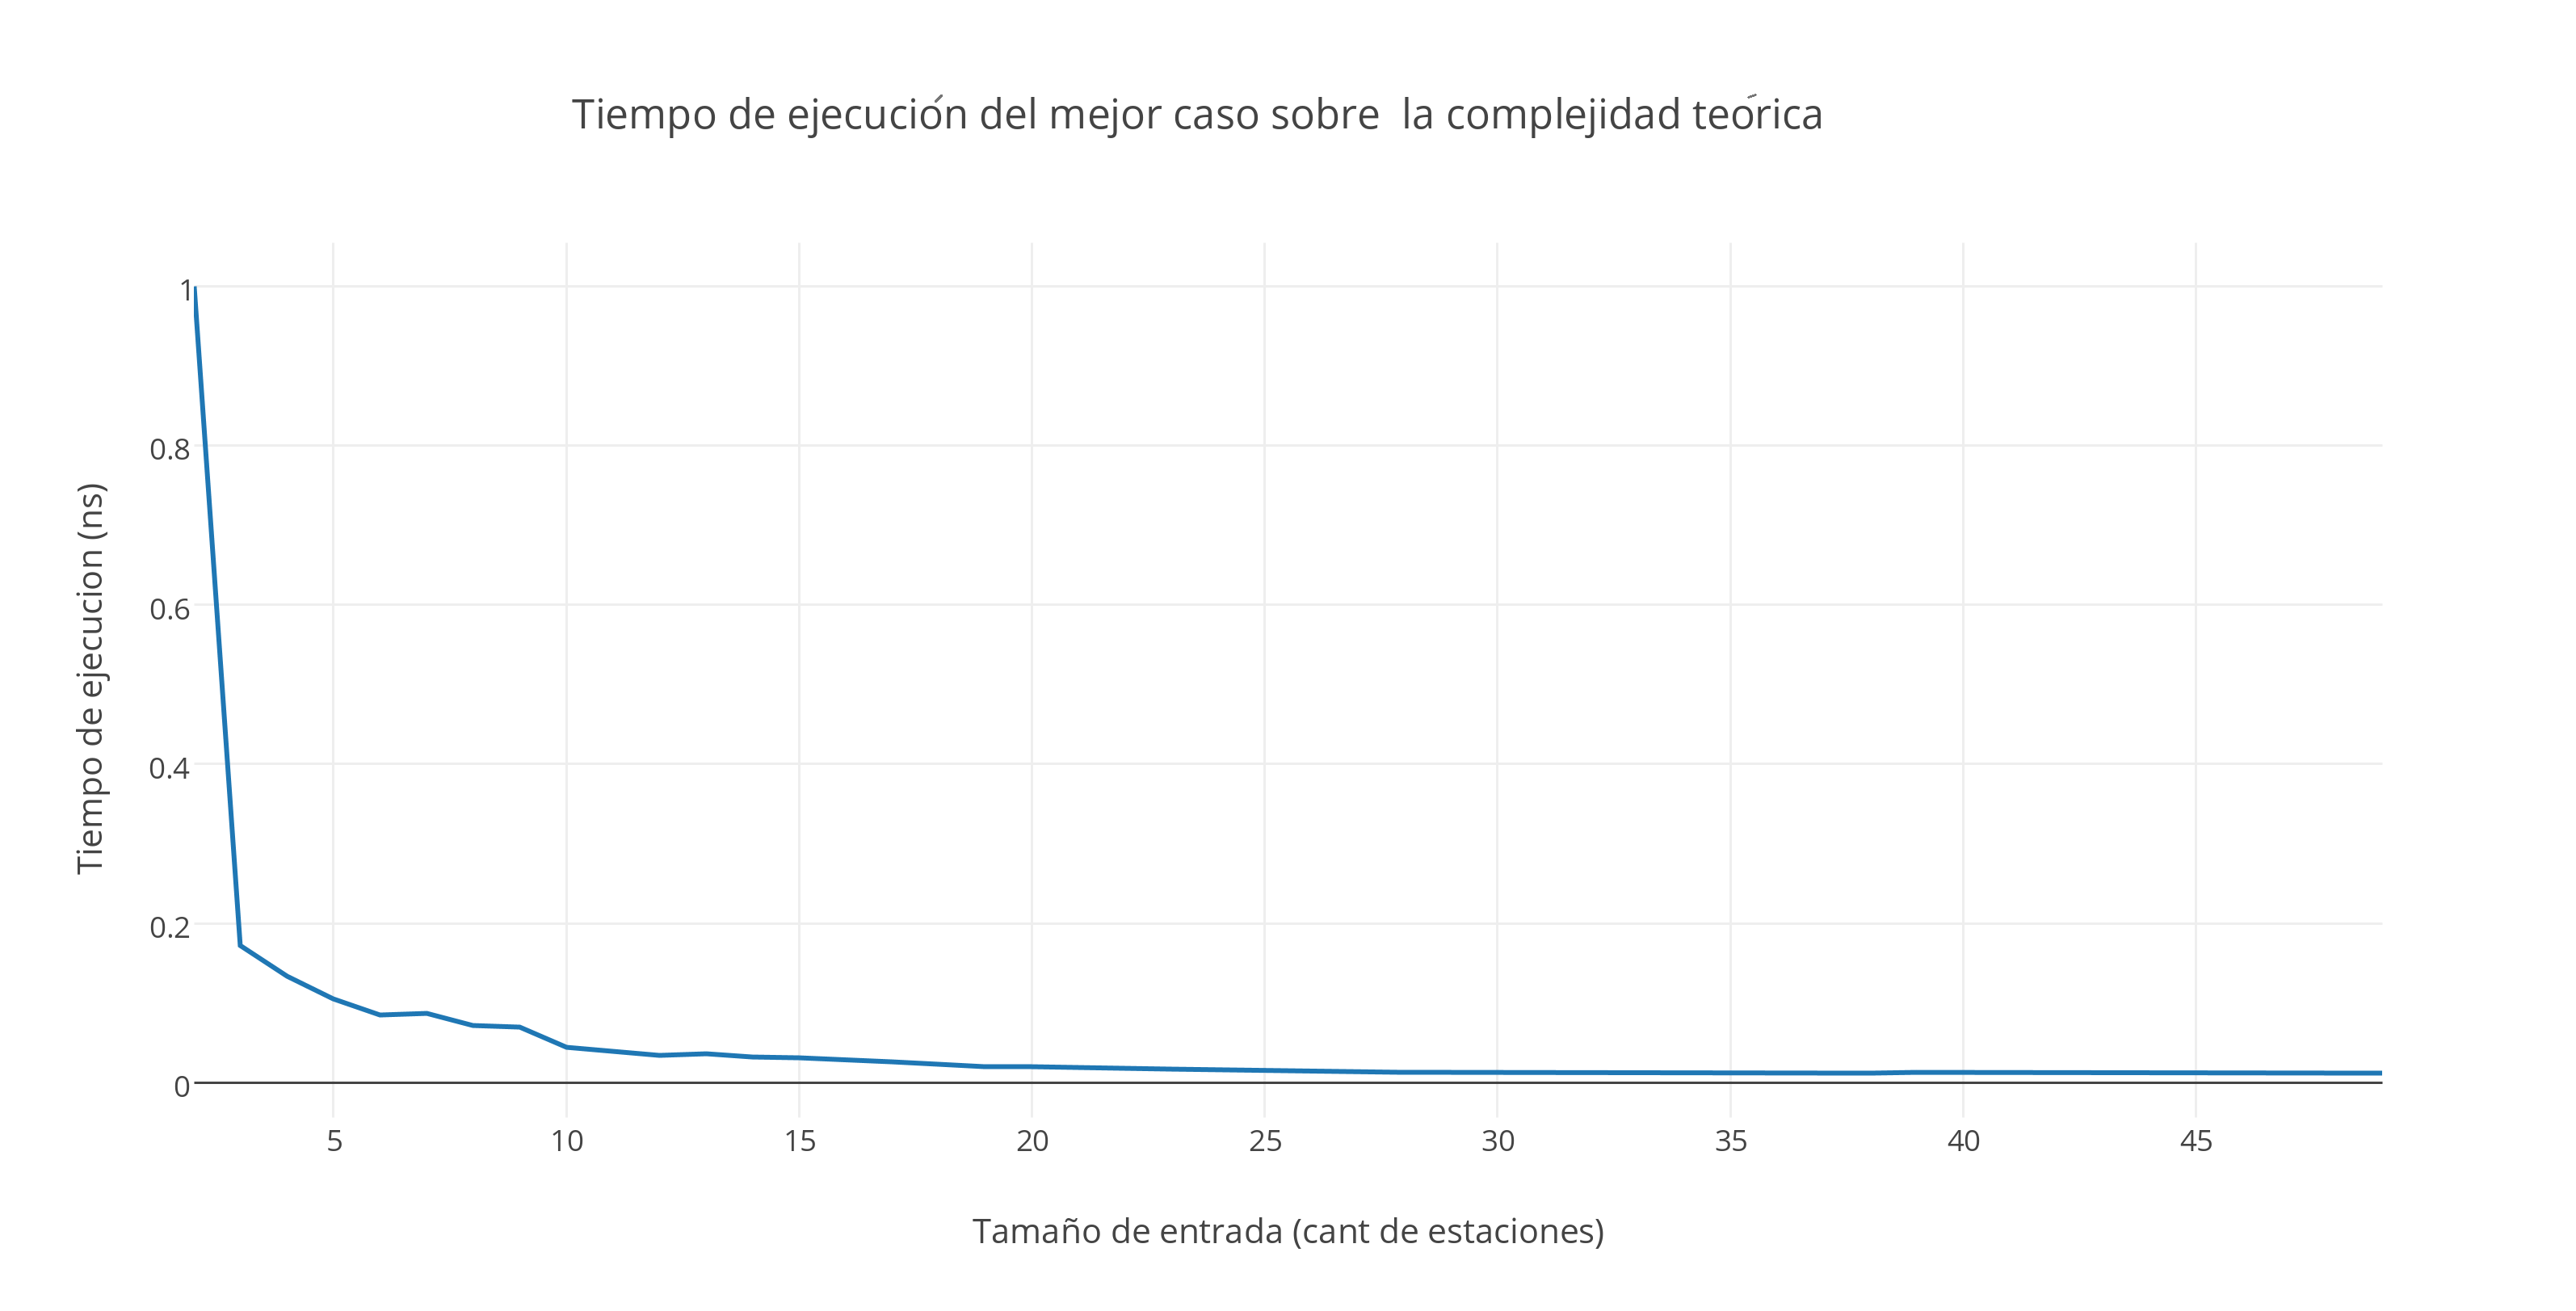
\includegraphics[scale=0.65]{./EJ3/mejorcaso2.png}
{$Gr$\'a$fico$ \ 3.4 - $Mejor$ $Caso$ / $Complejidad$ $O(N^2)$}
  \end{center}
  \vspace*{0.3cm}

Para realizar esta experimentaci\'on nos parecio prudente, realizar un promedio con el mismo input de aproximadamente 20 corridas
tanto para la complejidad como para nuestro algoritmo y una vez calculado dicho promedio de ambas cosas realizamos la divisi\'on para
obtener resultados m\'as relevantes.\\ 

Se puede observar en el gr\'afico 3.4, como luego de realizar la divisi\'on por la complejidad se ve que la funci\'on resultante tiende a 0 ya que nuestro algoritmo en este tipo de casa trabaja en el orden de O(N) lo cual es mucho menos que la complejidad te\'orica. Por lo tanto, podemos concluir que para el mejor caso nuestro algoritmo se encuentra considerablemente por debajo de la cota teorica $O(N^2)$.\\

Luego, verificando el peor caso, llegamos a la conclusi\'on que la familia de casos en el que resulta menos beneficioso trabajar con nuestro algoritmo ser\'a cuando \textbf{el grafo que se obtiene de transformar el circuito de estaciones de entrada es aquel que presenta multiples caminos para llegar a destino donde la suma de estos caminos presentan el mismo valor}, dandonos el siguiente grafo una vez transformado:\\


\vspace*{0.3cm} \vspace*{0.3cm}
  \begin{center}
 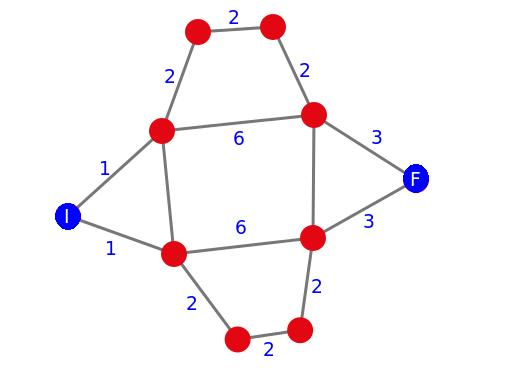
\includegraphics[scale=0.5]{./EJ3/grafoMultiCamino.jpeg}
 \\{$Grafo$ \ 3.2 - $Peor$ $Caso$}
  \end{center}
  \vspace*{0.3cm}
  
Realizando experimentos con un total de 50 instancias, desarrollamos dos gr\'aficos los cuales mostraremos a continuaci\'on: \\

\vspace*{0.3cm} \vspace*{0.3cm}
  \begin{center}
 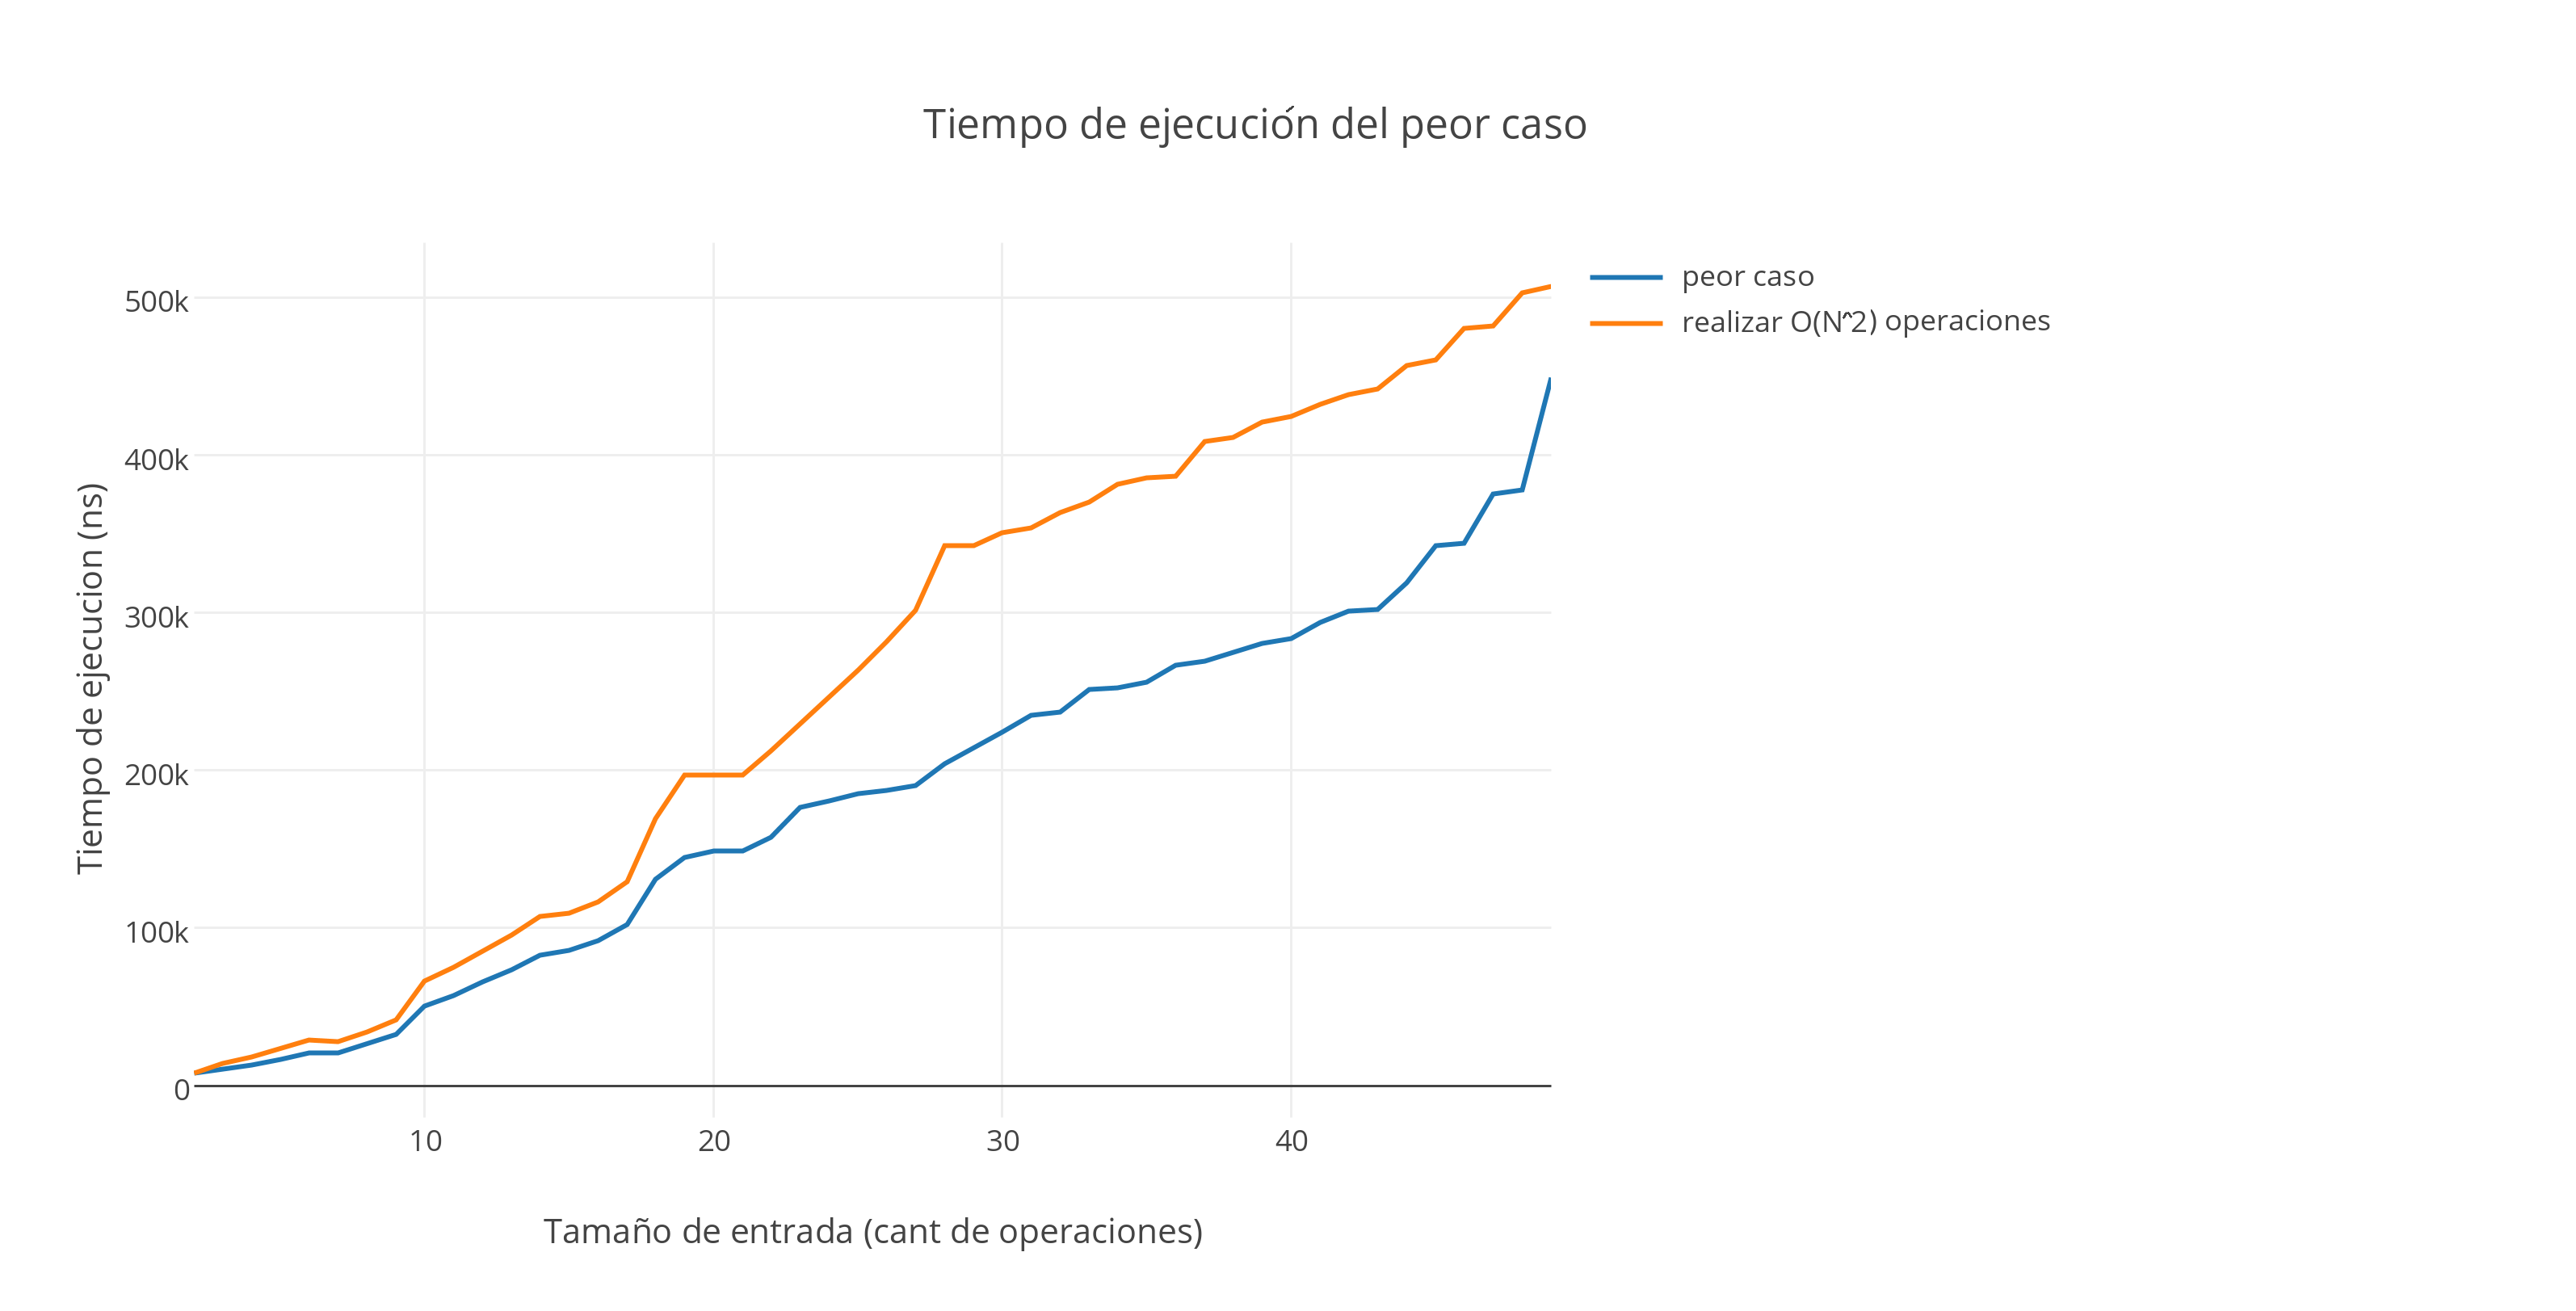
\includegraphics[scale=0.65]{./EJ3/peorcaso.png}
 {$Gr$\'a$fico$ \ 3.5 - $Peor$ $Caso$}
  \end{center}
  \vspace*{0.3cm}


Dividiendo por la complejidad propuesta llegamos a:\\

\vspace*{0.3cm} \vspace*{0.3cm}
  \begin{center}
 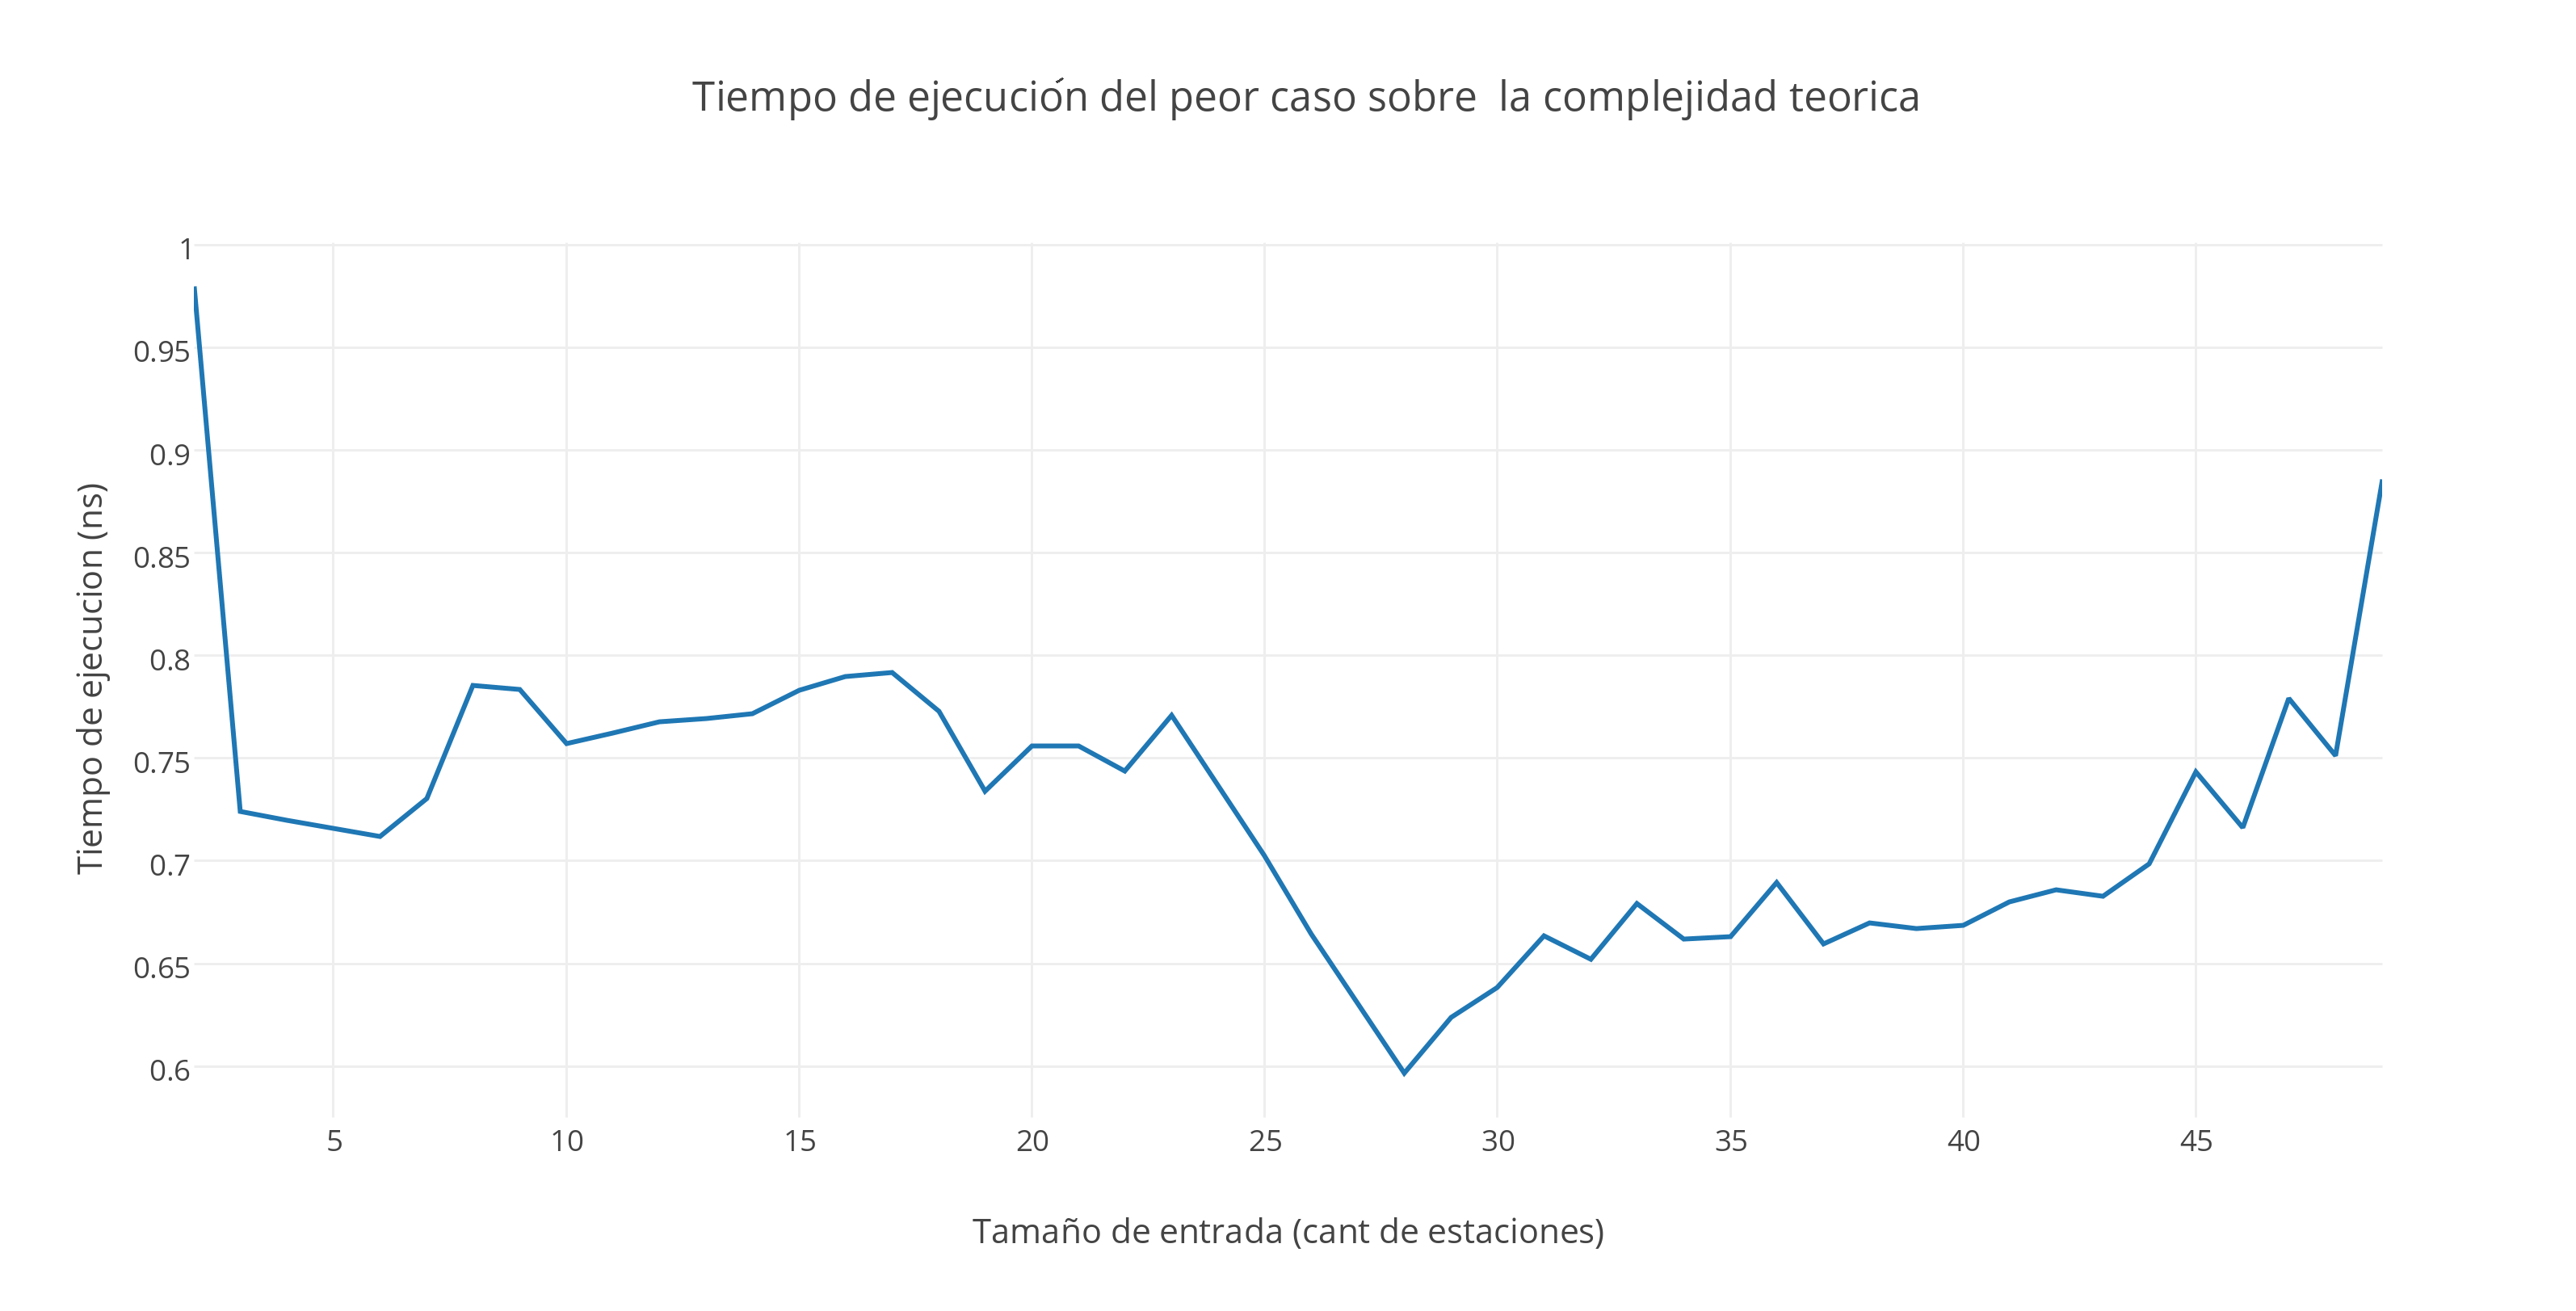
\includegraphics[scale=0.65]{./EJ3/peorcaso1.png}
 {$Gr$\'a$fico$ \ 3.6 - $Peor$ $Caso$ / $Complejidad$ $O(N^2)$}
  \end{center}
  \vspace*{0.3cm}

Para realizar esta experimentaci\'on nos parecio acorde, realizar un promedio con el mismo input de aproximadamente 20 corridas
tanto para la complejidad como para nuestro algoritmo y una vez calculado dicho promedio de ambas cosas realizamos la divisi\'on para
obtener resultados m\'as relevantes.\\ 

Como se puede observar en el gr\'afico 3.5, la funci\'on resultante de nuestro algoritmo es considerablemente mejor que la de la cota teorica  y presenta un tiempo similar al de la funci\'on resultante de la cota.
Luego, en el gr\'afico 3.6 se ve como la función resultante presenta un m\'aximo muy cerca de 1 y cuando el N aumenta la misma tiende a 0.\\

Por \'ultimo, mostraremos un gr\'afico comparativo entre el mejor y peor caso contra la complejidad que se solicito:\\

\vspace*{0.3cm} \vspace*{0.3cm}
  \begin{center}
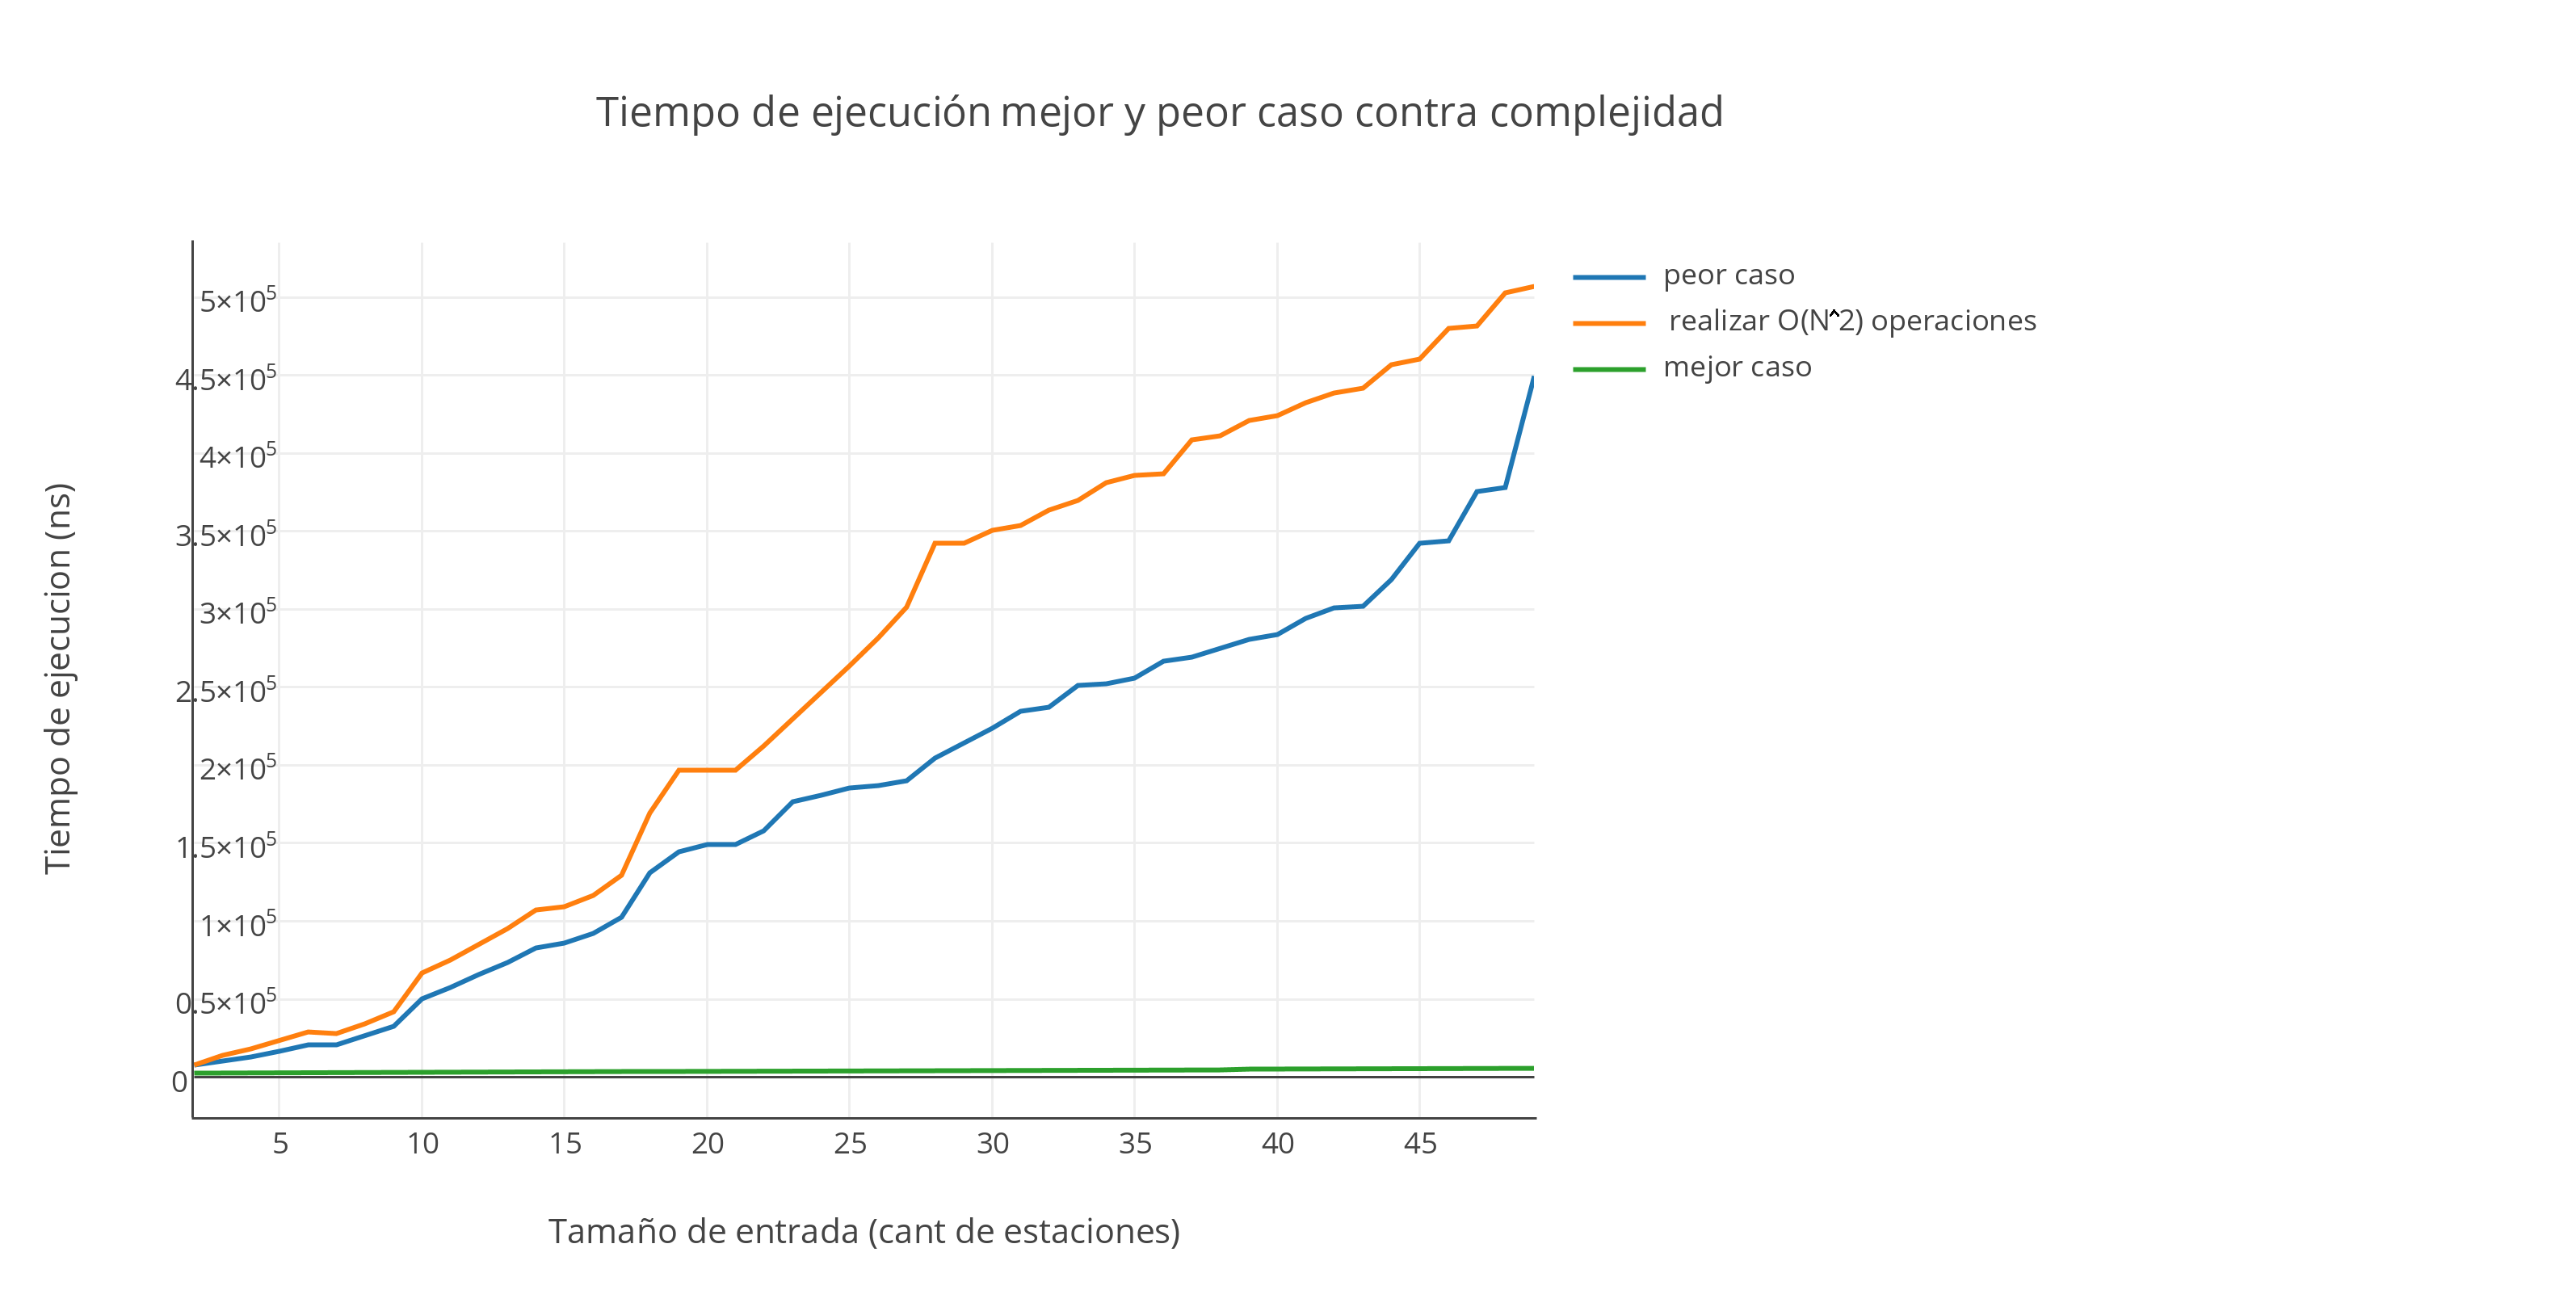
\includegraphics[scale=0.65]{./EJ3/comparativo1.png}
 {$Gr$\'a$fico$ \ 3.7 - $Comparativo$}
  \end{center}
  \vspace*{0.3cm}
  
Luego de dichos experimentos y casos probados, se puede concluir que a pesar de tener ciclos en todas las salas y donde dichos ciclos presenten aristas con pesos iguales lo que generara al algoritmo la posibilidad de crear varias ramas posibles de soluci\'on nos mantenemos dentro de la complejidad propuesta como hab\'iamos mostrado en nuestro desarrollo de la complejidad.\\
